\section{Métodos}

El proyecto se enfoca en mejorar imágenes mediante preprocesamiento, reducción de ruido y optimización visual. Se inició con 28 imágenes exploratorias para pruebas antes de aplicarlo a un conjunto de datos mayor.  Primero, se verifican el tipo y dimensiones de cada imagen. Luego, se convierten a escala de grises para simplificar el análisis y reducir la complejidad computacional, ajustándolas al formato unit8 sin pérdida de información. Después, se genera el histograma de intensidad para analizar contraste y distribución de píxeles. Luego, se aplica la ecualización del histograma para mejorar la visibilidad. Para reducir ruido y resaltar detalles, se usan filtros como el bilateral, que suaviza sin perder bordes, y el laplaciano, que enfatiza contornos. Un proceso automatizado aplica estos pasos a todas las imágenes.
Los resultados se evalúan comparando imágenes originales y procesadas. Se prueban combinaciones adicionales de filtros, como el de mediana y el gaussiano, para optimizar la nitidez. Esta fase exploratoria garantiza la efectividad del método antes de su aplicación en un conjunto de datos mayor.

Para llevar a cabo este proceso, se utilizan diversas herramientas y bibliotecas especializadas en procesamiento de imágenes y análisis de datos, las cuales están alineadas con los objetivos del proyecto optimizando tiempo de procesamiento por medio de la automatización. Algunas de las herramientas clave incluyen:
\begin{itemize}
    \item \textbf{Python}: El lenguaje de programación utilizado para implementar la solución.
    \item \textbf{OpenCV}: Biblioteca para el procesamiento de imágenes.
    \item \textbf{Matplotlib}: Utilizada para visualizar y comparar las imágenes procesadas.
    \item \textbf{NumPy}: Biblioteca esencial para la manipulación de matrices.
\end{itemize}

Adicionalmente, el flujo de trabajo (Figura 1) asegura que las imágenes sean procesadas de manera eficiente y efectiva, permitiendo mejorar su calidad visual y, al mismo tiempo, optimizar el tiempo de procesamiento a través de la automatización de tareas repetitivas. Las imágenes exploratorias sirven como un paso intermedio para validar las técnicas antes de aplicar el proceso al conjunto de datos completo.

\begin{figure}
    \centering
    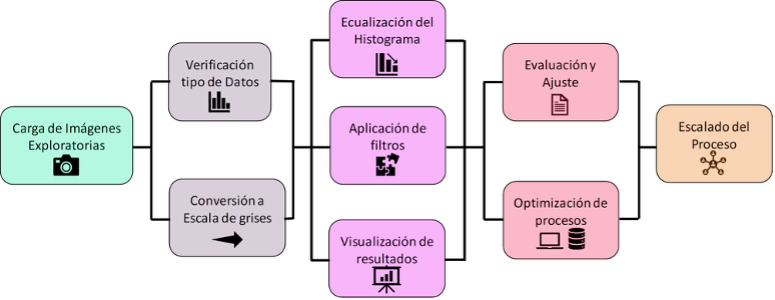
\includegraphics[width=0.4\textwidth]{figures/flujo.png}
    \caption{Flujo de trabajo para el procesamiento de imágenes.}
    \label{fig:flujo_trabajo}
\end{figure}